\chapter{Freedom From Violence}

This chapter is based on J. Krishnamurti's 1970 San Diego discussion with students, preserved in the Krishnamurti Foundation Trust source material and curated for this course by LazyingArt LLC through Video2Book. The lecture has no validated blackboard frames, visible equations, or diagram screenshots. The mathematics below is therefore deliberately modest: transcript-derived notation for the logic of the inquiry, not a physics model and not a formal psychology. We use it to keep the movement clear: dialogue rather than opinion, war as the opening pressure, the me as centre, cause becoming effect, naming as the past entering the present, image-making through inattention, and the final refusal of any formula for non-violence.

\section{Dialogue, Defensive War, and the Question Beneath It}

Krishnamurti begins by questioning the form of the meeting before taking up its content. A discussion, if it means an exchange of opinions, will not do. Opinion, intellectual cleverness, emotional reaction, and sentimental agreement are not the ground of this inquiry. The question has to arise from daily living, where conflict, fear, belief, desire, and relationship are actually taking place.

That opening is not a preface. It is the rule of motion for the whole lecture. Whenever the conversation drifts toward a theory, a label, or a defended position, Krishnamurti returns it to the fact: violence in oneself, violence in relationship, violence in the mind that divides.

The first student gives the inquiry its concrete pressure. He says, in effect, that he does not kill, yet asks whether war against communism may be justified as self-protection. Krishnamurti does not answer by comparing political systems. He notices the structure of the justification: every war is called self-protective by those who conduct it. If we accept the label too quickly, the inquiry is already over. So he pivots from the defence of a particular war to the deeper question: what is violence in the human being, and can the mind be free of it?

\subsection{Question \& Answer}

\paragraph{Question.}
Is war, when called self-protection, something different from violence?

\paragraph{Answer.}
No decisive inquiry begins by accepting the word self-protection. Krishnamurti points out that every war is so described by its makers. Whether the war is called offensive or defensive, it remains war. The useful question is not whether the label can be justified, but whether we can look at aggression and violence without hiding them behind the label.

\section{The Whole Spectrum and the Centre Called the Me}

The first expansion is from obvious violence to the whole spectrum. Violence is not only killing or war. It includes aggression, competition, the drive to become somebody, discipline according to a pattern, suppression, bullying oneself, and the inward brutality of forcing oneself toward an image.

A compact notation for the field is:
\begin{equation}
\mathcal{V}
=
\{\text{war},\ \text{killing},\ \text{aggression},\ \text{competition},\ \text{becoming},\ \text{suppression},\ \text{resistance}\}.
\end{equation}
Here \(\mathcal{V}\) is not a formal set in a technical theory. It is a reader's shorthand for the range Krishnamurti opens before asking whether we will look at violence bit by bit or as a whole.

When a student asks for the source, Krishnamurti names the centre: the me, the ego, the self. But he does not leave it as a doctrine. The me is shown in motion. It divides: me and not-me, conscious and unconscious, family and not-family, community and not-community. Like a stone dropped into a lake, the centre sends out waves.

\begin{equation}
\text{me}
\rightarrow
\{\text{me/not-me},\ \text{family/not-family},\ \text{community/not-community},\ \text{nation/nation},\ \text{belief/belief}\}.
\end{equation}

The point sharpens at once. The me is not merely private, and society is not merely outside us. We have built a violent society, and that society has shaped us. If we split the individual from culture too cleanly, we repeat the very division we are trying to understand.

\begin{figure}
\centering
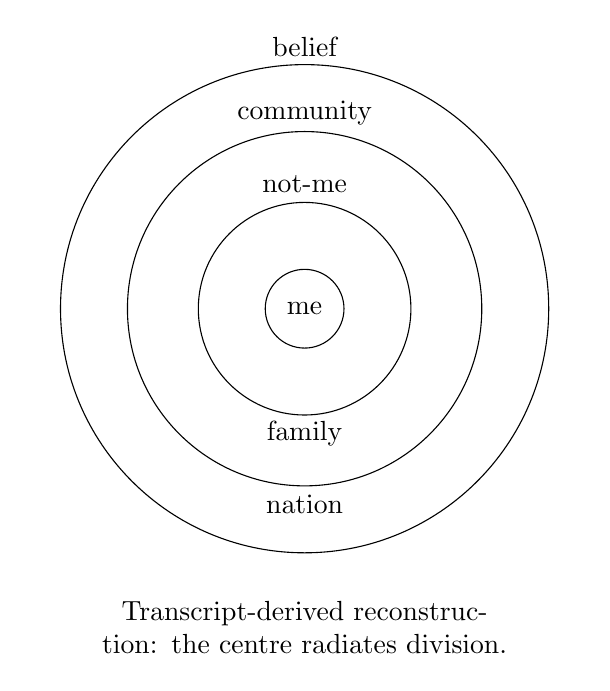
\begin{tikzpicture}[scale=1]
\node[draw, circle, minimum size=1.0cm] (me) at (0,0) {me};
\draw (0,0) circle (1.35cm);
\draw (0,0) circle (2.25cm);
\draw (0,0) circle (3.10cm);
\node[text width=2.2cm, align=center] at (0,1.58) {not-me};
\node[text width=2.2cm, align=center] at (0,-1.58) {family};
\node[text width=2.2cm, align=center] at (0,2.48) {community};
\node[text width=2.2cm, align=center] at (0,-2.48) {nation};
\node[text width=2.2cm, align=center] at (0,3.33) {belief};
\node[text width=6.8cm, align=center] at (0,-4.05)
{Transcript-derived reconstruction: the centre radiates division.};
\end{tikzpicture}
\end{figure}

So the lecture has already moved through three levels: political violence, inward violence, and the centre that divides. The next move is subtler. Even if we have named the centre, has naming the cause ended violence?

\section{Cause, Effect, and the Refusal to Chase the Chain}

Krishnamurti pauses over a common assumption: if I know why I am brutal, I will be finished with brutality. He rejects that confidence. One may search for causes, consult explanations, gather theories, and still remain violent.

The reason is not that causes do not matter. It is that cause and effect are not sharply separated in the movement of life. A cause becomes an effect; that effect becomes a new cause; the chain continues.

\begin{equation}
C \rightarrow E \rightarrow C' \rightarrow E' \rightarrow \cdots
\end{equation}

A compact update rule makes the recurrence visible:
\begin{align}
C_{n+1} &= E_n,\\
E_{n+1} &= f(C_{n+1}).
\end{align}
In this notation \(C\) means cause and \(E\) means effect. The function \(f\) is only a schematic placeholder for ``what follows from.'' Nothing in the transcript warrants a formal causal calculus. The notation simply preserves the lecture's warning: an explanatory chain can be extended indefinitely while the fact remains untouched.

\subsection{Question \& Answer}

\paragraph{Question.}
Does finding the cause of violence end violence?

\paragraph{Answer.}
No. The discovery of a cause can become another postponement. Krishnamurti says that the cause becomes the effect and the effect becomes the cause. Therefore the inquiry cannot be satisfied by explanation. It must look at violence as a whole, including the me and the society it both makes and inherits.

\begin{proposition}
In the lecture's logic, causal explanation is insufficient when it becomes a substitute for direct observation.
\end{proposition}

\begin{proof}
The reasoning is short.
\begin{enumerate}
\item We begin with the fact of violence.
\item We ask for a cause.
\item The named cause becomes part of the next state of the problem.
\item That next state produces further effects, which become further causes.
\item Thus the cause-effect sequence may continue without ending violence.
\item Therefore explanation must give way to seeing the whole movement directly.
\end{enumerate}
\end{proof}

This is the first worked structure of the chapter. It is not a derivation from axioms. It is a disciplined way to keep the lecture's transition clear: from explanation to looking.

\section{Recognition, Naming, and the Past}

The question now changes. We are no longer asking only what violence is. Krishnamurti asks: how do we know we are violent?

He begins with a simple example. I am angry. At the exact moment of anger, recognition may not yet have occurred. A moment later thought says, ``I have been angry.'' That recognition is possible only because anger has been known before. The past enters and names the present.

\begin{equation}
\text{present response}+\text{memory}
\rightarrow
\text{recognition/name}.
\end{equation}

This is the lecture's central turn toward thought, time, and image. Naming is not neutral. It relates the present response to the past. The mind then looks with eyes already touched by condemnation, justification, explanation, or habit.

The movement away from the fact can be recorded as:
\begin{equation}
\text{fact}
\rightarrow
\text{name}
\rightarrow
\text{past}
\rightarrow
\text{escape from the fact}.
\end{equation}

Krishnamurti extends the same point through loneliness and the tree. If I say, ``I am lonely,'' the word may already be a movement away. If I look at a tree and immediately say it is beautiful, the word has already interrupted looking. The issue is not that words are forbidden. The issue is that the word is not the thing, the description is not the described, and the explanation is not the explained.

\begin{table}
\centering
\begin{tabular}{p{0.42\linewidth}p{0.42\linewidth}}
Movement away from the fact & Direct looking in the lecture's sense \\
\hline
seeking the cause & seeing the whole movement \\
naming & looking without the past taking charge \\
condemning or justifying & remaining with what is \\
exercise of will & attention not born of resistance \\
belief or formula & seeing danger directly \\
\end{tabular}
\end{table}

The table is only a pocket map. The lecture itself moves more slowly because the difficulty is real: all our living is burdened by the past.

\section{Image, Relationship, and Attention}

Krishnamurti next gives the recognition problem a relational form. Someone calls me a fool. The body and nerves react, but what is really touched is the image I have of myself. That image says, ``I am not a fool.'' The old responds.

From there he moves to husband and wife. Do I ever look directly at the other person, or do I look through the image I have built across years? If the other person does the same, then what we call relationship is not actual relationship. It is image meeting image.

\begin{equation}
\text{image}_A \leftrightarrow \text{image}_B
\neq
\text{actual relationship}.
\end{equation}

\subsection{Question \& Answer}

\paragraph{Question.}
How is the image formed?

\paragraph{Answer.}
The student suggests that there is space between perception and response, perhaps time. Krishnamurti accepts the direction and makes it concrete. Insult or flattery leaves a mark when there is inattention. Repeated marks become images. But when there is attention at the moment of insult or flattery, there is no marking.

\begin{equation}
\text{insult/flattery}+\text{inattention}
\rightarrow
\text{mark}
\rightarrow
\text{image}.
\end{equation}

\begin{equation}
\text{insult/flattery}+\text{attention}
\rightarrow
\text{no mark}.
\end{equation}

\begin{figure}
\centering
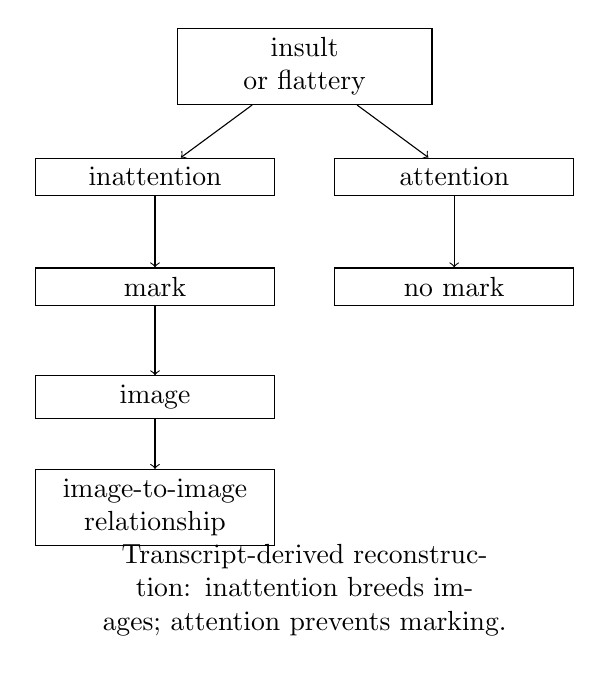
\begin{tikzpicture}[scale=1]
\node[draw, rectangle, text width=3.0cm, align=center] (event) at (0,3.2) {insult\\or flattery};

\node[draw, rectangle, text width=2.8cm, align=center] (inatt) at (-1.9,1.8) {inattention};
\node[draw, rectangle, text width=2.8cm, align=center] (att) at (1.9,1.8) {attention};

\node[draw, rectangle, text width=2.8cm, align=center] (mark) at (-1.9,0.4) {mark};
\node[draw, rectangle, text width=2.8cm, align=center] (image) at (-1.9,-1.0) {image};
\node[draw, rectangle, text width=2.8cm, align=center] (rel) at (-1.9,-2.4) {image-to-image\\relationship};

\node[draw, rectangle, text width=2.8cm, align=center] (nomark) at (1.9,0.4) {no mark};

\draw[->] (event) -- (inatt);
\draw[->] (event) -- (att);
\draw[->] (inatt) -- (mark);
\draw[->] (mark) -- (image);
\draw[->] (image) -- (rel);
\draw[->] (att) -- (nomark);

\node[text width=6.8cm, align=center] at (0,-3.45)
{Transcript-derived reconstruction: inattention breeds images; attention prevents marking.};
\end{tikzpicture}
\end{figure}

This is a decisive distinction, but it must not be turned into a method. The next question asks whether attention is an act of will, and Krishnamurti says no. Will is precisely the next structure to be examined.

\section{Will, Frustration, Resistance, and Energy}

The student asks whether attention is an act of will. Krishnamurti replies by asking what will is: I want, I will, I shall, I demand. Will is desire taking the form of resistance. And resistance is violence.

\begin{equation}
\text{will}
\sim
\text{desire}+\text{demand}+\text{resistance}.
\end{equation}

\begin{equation}
\text{resistance}
\rightarrow
\text{division}
\rightarrow
\text{violence}.
\end{equation}

This explains why the lecture will not prescribe a technique for attention. A technique held by will would belong to the same movement of demand and resistance.

The same pattern appears in frustration. A student asks whether some violence might be healthy, meaning frustration rather than physical attack. Krishnamurti turns the question: what is fulfilment, and who is fulfilling? The answer again returns to the me. The me seeks expansion, achievement, fame, importance. When expansion is blocked, frustration appears; frustration becomes bitterness; bitterness is violence.

\begin{equation}
\text{me seeks expansion}
\rightarrow
\text{frustration}
\rightarrow
\text{bitterness}
\rightarrow
\text{violence}.
\end{equation}

Late in the dialogue, the word energy becomes important. Krishnamurti says violence is a form of energy. Love surrounded by jealousy, anxiety, fear, and bitterness is also caught in energy. Resistance wastes energy because it breeds division. Seeing the truth of resistance changes the movement of energy.

We should keep this language close to the source. It is not a conservation law. It is not a physical transformation rule. It is a way of saying that the force now moving as aggression, jealousy, fear, or division is not to be manipulated by formula, but understood without resistance.

\section{Belief, Freedom, and Meeting Violence in Another}

The last movement of the dialogue is not a clean lecture-room conclusion. It is a sequence of tests. Students ask about animals, language, psychic experience, belief, unity, freedom, purpose, logic, intuition, and how to meet another person's violence. Each time Krishnamurti brings the conversation back to the fact of violence and the danger of moving away from it through words, beliefs, or formulas.

Belief is treated as division. One person has one belief, another has another belief, and human beings fight over belief. Even belief in unity remains belief if it is not fact. The relevant notation is blunt:
\begin{equation}
\text{belief}
\rightarrow
\text{division}
\rightarrow
\text{violence}.
\end{equation}

Freedom receives the same treatment. The student asks about freedom from and freedom to. Krishnamurti refuses both formulations. Freedom is not a movement away from one object or toward another. Freedom is freedom.

Purpose is also brought under the inquiry. If each person or group has its own psychological purpose, that purpose divides. The religious man has one purpose, the scientist another, the family another. The point is not to deny ordinary practical functioning. The point is that purpose held by the me can become another centre of division.

The most practical late question returns us to the opening. How do we meet violence in another? Krishnamurti does not offer a rule. He asks whether the question would arise in the same way if there were no violence in oneself. If there is no hatred, no bitterness, no fulfilment-seeking, no desire to become, then one will know what to do when the neighbour is violent. Another person may call the action violent, but that judgment is secondary to the fact of whether there is violence in one's own heart and mind.

The closing warning is the final equation of the lecture:
\begin{equation}
\text{formula for non-violence}
\rightarrow
\text{violence}.
\end{equation}

To determine in advance how one will act non-violently is already to build a formula. The formula belongs to thought, will, image, and becoming. Krishnamurti ends by refusing that movement.

\section{Summary}

The lecture begins with a student's question about justified war and ends by rejecting every formula for non-violence. Its order matters. War opens the door, but the inquiry immediately widens to the whole spectrum of violence: aggression, competition, becoming, suppression, discipline according to a pattern, and inward brutality. The me is then named as the centre from which division radiates, but even that naming is not allowed to become a final explanation.

The cause-effect chain shows why explanation alone is insufficient: cause becomes effect, effect becomes cause, and the mind can continue indefinitely while remaining violent. The deeper turn is toward recognition, naming, image, and attention. Naming brings the past into the present. Inattention leaves marks. Marks accumulate as images. Images replace relationship.

The later questions test the same insight. Will is resistance; resistance breeds division; frustration is the me seeking expansion; belief divides; freedom is not from or to; and a formula for non-violence breeds violence. The chapter's formulas and diagrams are only compact aids. The source remains the living inquiry: can violence be seen as a whole, without escape, without naming, without justification, without condemnation, and without the mind preparing an image of what it will become?